
%% bare_conf.tex
%% V1.3
%% 2007/01/11
%% by Michael Shell
%% See:
%% http://www.michaelshell.org/
%% for current contact information.
%%
%% This is a skeleton file demonstrating the use of IEEEtran.cls
%% (requires IEEEtran.cls version 1.7 or later) with an IEEE conference paper.
%%
%% Support sites:
%% http://www.michaelshell.org/tex/ieeetran/
%% http://www.ctan.org/tex-archive/macros/latex/contrib/IEEEtran/
%% and
%% http://www.ieee.org/

%%*************************************************************************
%% Legal Notice:
%% This code is offered as-is without any warranty either expressed or
%% implied; without even the implied warranty of MERCHANTABILITY or
%% FITNESS FOR A PARTICULAR PURPOSE! 
%% User assumes all risk.
%% In no event shall IEEE or any contributor to this code be liable for
%% any damages or losses, including, but not limited to, incidental,
%% consequential, or any other damages, resulting from the use or misuse
%% of any information contained here.
%%
%% All comments are the opinions of their respective authors and are not
%% necessarily endorsed by the IEEE.
%%
%% This work is distributed under the LaTeX Project Public License (LPPL)
%% ( http://www.latex-project.org/ ) version 1.3, and may be freely used,
%% distributed and modified. A copy of the LPPL, version 1.3, is included
%% in the base LaTeX documentation of all distributions of LaTeX released
%% 2003/12/01 or later.
%% Retain all contribution notices and credits.
%% ** Modified files should be clearly indicated as such, including  **
%% ** renaming them and changing author support contact information. **
%%
%% File list of work: IEEEtran.cls, IEEEtran_HOWTO.pdf, bare_adv.tex,
%%                    bare_conf.tex, bare_jrnl.tex, bare_jrnl_compsoc.tex
%%*************************************************************************

% *** Authors should verify (and, if needed, correct) their LaTeX system  ***
% *** with the testflow diagnostic prior to trusting their LaTeX platform ***
% *** with production work. IEEE's font choices can trigger bugs that do  ***
% *** not appear when using other class files.                            ***
% The testflow support page is at:
% http://www.michaelshell.org/tex/testflow/



% Note that the a4paper option is mainly intended so that authors in
% countries using A4 can easily print to A4 and see how their papers will
% look in print - the typesetting of the document will not typically be
% affected with changes in paper size (but the bottom and side margins will).
% Use the testflow package mentioned above to verify correct handling of
% both paper sizes by the user's LaTeX system.
%
% Also note that the "draftcls" or "draftclsnofoot", not "draft", option
% should be used if it is desired that the figures are to be displayed in
% draft mode.
%
\documentclass[conference]{IEEEtran}
\usepackage{blindtext, graphicx}
\usepackage{amsmath}
\usepackage{algorithm}
\usepackage[noend]{algpseudocode}

\usepackage{mathtools,xparse}

\DeclarePairedDelimiter{\abs}{\lvert}{\rvert}
\DeclarePairedDelimiter{\norm}{\lVert}{\rVert}
\NewDocumentCommand{\normL}{ s O{} m }{%
  \IfBooleanTF{#1}{\norm*{#3}}{\norm[#2]{#3}}_{L_2(\Omega)}%
}
% Add the compsoc option for Computer Society conferences.
%
% If IEEEtran.cls has not been installed into the LaTeX system files,
% manually specify the path to it like:
% \documentclass[conference]{../sty/IEEEtran}





% Some very useful LaTeX packages include:
% (uncomment the ones you want to load)


% *** MISC UTILITY PACKAGES ***
%
%\usepackage{ifpdf}
% Heiko Oberdiek's ifpdf.sty is very useful if you need conditional
% compilation based on whether the output is pdf or dvi.
% usage:
% \ifpdf
%   % pdf code
% \else
%   % dvi code
% \fi
% The latest version of ifpdf.sty can be obtained from:
% http://www.ctan.org/tex-archive/macros/latex/contrib/oberdiek/
% Also, note that IEEEtran.cls V1.7 and later provides a builtin
% \ifCLASSINFOpdf conditional that works the same way.
% When switching from latex to pdflatex and vice-versa, the compiler may
% have to be run twice to clear warning/error messages.






% *** CITATION PACKAGES ***
%
%\usepackage{cite}
% cite.sty was written by Donald Arseneau
% V1.6 and later of IEEEtran pre-defines the format of the cite.sty package
% \cite{} output to follow that of IEEE. Loading the cite package will
% result in citation numbers being automatically sorted and properly
% "compressed/ranged". e.g., [1], [9], [2], [7], [5], [6] without using
% cite.sty will become [1], [2], [5]--[7], [9] using cite.sty. cite.sty's
% \cite will automatically add leading space, if needed. Use cite.sty's
% noadjust option (cite.sty V3.8 and later) if you want to turn this off.
% cite.sty is already installed on most LaTeX systems. Be sure and use
% version 4.0 (2003-05-27) and later if using hyperref.sty. cite.sty does
% not currently provide for hyperlinked citations.
% The latest version can be obtained at:
% http://www.ctan.org/tex-archive/macros/latex/contrib/cite/
% The documentation is contained in the cite.sty file itself.






% *** GRAPHICS RELATED PACKAGES ***
%
\ifCLASSINFOpdf
  % \usepackage[pdftex]{graphicx}
  % declare the path(s) where your graphic files are
  % \graphicspath{{../pdf/}{../jpeg/}}
  % and their extensions so you won't have to specify these with
  % every instance of \includegraphics
  % \DeclareGraphicsExtensions{.pdf,.jpeg,.png}
\else
  % or other class option (dvipsone, dvipdf, if not using dvips). graphicx
  % will default to the driver specified in the system graphics.cfg if no
  % driver is specified.
  % \usepackage[dvips]{graphicx}
  % declare the path(s) where your graphic files are
  % \graphicspath{{../eps/}}
  % and their extensions so you won't have to specify these with
  % every instance of \includegraphics
  % \DeclareGraphicsExtensions{.eps}
\fi
% graphicx was written by David Carlisle and Sebastian Rahtz. It is
% required if you want graphics, photos, etc. graphicx.sty is already
% installed on most LaTeX systems. The latest version and documentation can
% be obtained at: 
% http://www.ctan.org/tex-archive/macros/latex/required/graphics/
% Another good source of documentation is "Using Imported Graphics in
% LaTeX2e" by Keith Reckdahl which can be found as epslatex.ps or
% epslatex.pdf at: http://www.ctan.org/tex-archive/info/
%
% latex, and pdflatex in dvi mode, support graphics in encapsulated
% postscript (.eps) format. pdflatex in pdf mode supports graphics
% in .pdf, .jpeg, .png and .mps (metapost) formats. Users should ensure
% that all non-photo figures use a vector format (.eps, .pdf, .mps) and
% not a bitmapped formats (.jpeg, .png). IEEE frowns on bitmapped formats
% which can result in "jaggedy"/blurry rendering of lines and letters as
% well as large increases in file sizes.
%
% You can find documentation about the pdfTeX application at:
% http://www.tug.org/applications/pdftex





% *** MATH PACKAGES ***
%
%\usepackage[cmex10]{amsmath}
% A popular package from the American Mathematical Society that provides
% many useful and powerful commands for dealing with mathematics. If using
% it, be sure to load this package with the cmex10 option to ensure that
% only type 1 fonts will utilized at all point sizes. Without this option,
% it is possible that some math symbols, particularly those within
% footnotes, will be rendered in bitmap form which will result in a
% document that can not be IEEE Xplore compliant!
%
% Also, note that the amsmath package sets \interdisplaylinepenalty to 10000
% thus preventing page breaks from occurring within multiline equations. Use:
%\interdisplaylinepenalty=2500
% after loading amsmath to restore such page breaks as IEEEtran.cls normally
% does. amsmath.sty is already installed on most LaTeX systems. The latest
% version and documentation can be obtained at:
% http://www.ctan.org/tex-archive/macros/latex/required/amslatex/math/





% *** SPECIALIZED LIST PACKAGES ***
%
%\usepackage{algorithmic}
% algorithmic.sty was written by Peter Williams and Rogerio Brito.
% This package provides an algorithmic environment fo describing algorithms.
% You can use the algorithmic environment in-text or within a figure
% environment to provide for a floating algorithm. Do NOT use the algorithm
% floating environment provided by algorithm.sty (by the same authors) or
% algorithm2e.sty (by Christophe Fiorio) as IEEE does not use dedicated
% algorithm float types and packages that provide these will not provide
% correct IEEE style captions. The latest version and documentation of
% algorithmic.sty can be obtained at:
% http://www.ctan.org/tex-archive/macros/latex/contrib/algorithms/
% There is also a support site at:
% http://algorithms.berlios.de/index.html
% Also of interest may be the (relatively newer and more customizable)
% algorithmicx.sty package by Szasz Janos:
% http://www.ctan.org/tex-archive/macros/latex/contrib/algorithmicx/




% *** ALIGNMENT PACKAGES ***
%
%\usepackage{array}
% Frank Mittelbach's and David Carlisle's array.sty patches and improves
% the standard LaTeX2e array and tabular environments to provide better
% appearance and additional user controls. As the default LaTeX2e table
% generation code is lacking to the point of almost being broken with
% respect to the quality of the end results, all users are strongly
% advised to use an enhanced (at the very least that provided by array.sty)
% set of table tools. array.sty is already installed on most systems. The
% latest version and documentation can be obtained at:
% http://www.ctan.org/tex-archive/macros/latex/required/tools/


%\usepackage{mdwmath}
%\usepackage{mdwtab}
% Also highly recommended is Mark Wooding's extremely powerful MDW tools,
% especially mdwmath.sty and mdwtab.sty which are used to format equations
% and tables, respectively. The MDWtools set is already installed on most
% LaTeX systems. The lastest version and documentation is available at:
% http://www.ctan.org/tex-archive/macros/latex/contrib/mdwtools/


% IEEEtran contains the IEEEeqnarray family of commands that can be used to
% generate multiline equations as well as matrices, tables, etc., of high
% quality.


%\usepackage{eqparbox}
% Also of notable interest is Scott Pakin's eqparbox package for creating
% (automatically sized) equal width boxes - aka "natural width parboxes".
% Available at:
% http://www.ctan.org/tex-archive/macros/latex/contrib/eqparbox/





% *** SUBFIGURE PACKAGES ***
%\usepackage[tight,footnotesize]{subfigure}
% subfigure.sty was written by Steven Douglas Cochran. This package makes it
% easy to put subfigures in your figures. e.g., "Figure 1a and 1b". For IEEE
% work, it is a good idea to load it with the tight package option to reduce
% the amount of white space around the subfigures. subfigure.sty is already
% installed on most LaTeX systems. The latest version and documentation can
% be obtained at:
% http://www.ctan.org/tex-archive/obsolete/macros/latex/contrib/subfigure/
% subfigure.sty has been superceeded by subfig.sty.



%\usepackage[caption=false]{caption}
%\usepackage[font=footnotesize]{subfig}
% subfig.sty, also written by Steven Douglas Cochran, is the modern
% replacement for subfigure.sty. However, subfig.sty requires and
% automatically loads Axel Sommerfeldt's caption.sty which will override
% IEEEtran.cls handling of captions and this will result in nonIEEE style
% figure/table captions. To prevent this problem, be sure and preload
% caption.sty with its "caption=false" package option. This is will preserve
% IEEEtran.cls handing of captions. Version 1.3 (2005/06/28) and later 
% (recommended due to many improvements over 1.2) of subfig.sty supports
% the caption=false option directly:
%\usepackage[caption=false,font=footnotesize]{subfig}
%
% The latest version and documentation can be obtained at:
% http://www.ctan.org/tex-archive/macros/latex/contrib/subfig/
% The latest version and documentation of caption.sty can be obtained at:
% http://www.ctan.org/tex-archive/macros/latex/contrib/caption/




% *** FLOAT PACKAGES ***
%
%\usepackage{fixltx2e}
% fixltx2e, the successor to the earlier fix2col.sty, was written by
% Frank Mittelbach and David Carlisle. This package corrects a few problems
% in the LaTeX2e kernel, the most notable of which is that in current
% LaTeX2e releases, the ordering of single and double column floats is not
% guaranteed to be preserved. Thus, an unpatched LaTeX2e can allow a
% single column figure to be placed prior to an earlier double column
% figure. The latest version and documentation can be found at:
% http://www.ctan.org/tex-archive/macros/latex/base/



%\usepackage{stfloats}
% stfloats.sty was written by Sigitas Tolusis. This package gives LaTeX2e
% the ability to do double column floats at the bottom of the page as well
% as the top. (e.g., "\begin{figure*}[!b]" is not normally possible in
% LaTeX2e). It also provides a command:
%\fnbelowfloat
% to enable the placement of footnotes below bottom floats (the standard
% LaTeX2e kernel puts them above bottom floats). This is an invasive package
% which rewrites many portions of the LaTeX2e float routines. It may not work
% with other packages that modify the LaTeX2e float routines. The latest
% version and documentation can be obtained at:
% http://www.ctan.org/tex-archive/macros/latex/contrib/sttools/
% Documentation is contained in the stfloats.sty comments as well as in the
% presfull.pdf file. Do not use the stfloats baselinefloat ability as IEEE
% does not allow \baselineskip to stretch. Authors submitting work to the
% IEEE should note that IEEE rarely uses double column equations and
% that authors should try to avoid such use. Do not be tempted to use the
% cuted.sty or midfloat.sty packages (also by Sigitas Tolusis) as IEEE does
% not format its papers in such ways.





% *** PDF, URL AND HYPERLINK PACKAGES ***
%
%\usepackage{url}
% url.sty was written by Donald Arseneau. It provides better support for
% handling and breaking URLs. url.sty is already installed on most LaTeX
% systems. The latest version can be obtained at:
% http://www.ctan.org/tex-archive/macros/latex/contrib/misc/
% Read the url.sty source comments for usage information. Basically,
% \url{my_url_here}.





% *** Do not adjust lengths that control margins, column widths, etc. ***
% *** Do not use packages that alter fonts (such as pslatex).         ***
% There should be no need to do such things with IEEEtran.cls V1.6 and later.
% (Unless specifically asked to do so by the journal or conference you plan
% to submit to, of course. )


% correct bad hyphenation here
\hyphenation{op-tical net-works semi-conduc-tor}


\begin{document}
%
% paper title
% can use linebreaks \\ within to get better formatting as desired
\title{Generic Game Playing Agent Using Deep Reinforcement Learning }


% author names and affiliations
% use a multiple column layout for up to three different
% affiliations
\author{\IEEEauthorblockN{Subhojeet}
\IEEEauthorblockA{Department of Computer Science\\
Indian Insitute of Technology\\
Guwahati, India\\
subhojeet@iitg.ernet.in}
\and
\IEEEauthorblockN{Dhruv Kohli}
\IEEEauthorblockA{Depratment of Mathematics\\
Indian Institute of Technology\\
Guwahati, India\\
dhruv.kohli@iitg.ernet.in}
\and
\IEEEauthorblockN{Dheeraj Khatri}
\IEEEauthorblockA{Department of Computer Science\\
Indian Insitute of Technology\\
Guwahati, India\\
d.khatri@iitg.ernet.in}}

% conference papers do not typically use \thanks and this command
% is locked out in conference mode. If really needed, such as for
% the acknowledgment of grants, issue a \IEEEoverridecommandlockouts
% after \documentclass

% for over three affiliations, or if they all won't fit within the width
% of the page, use this alternative format:
% 
%\author{\IEEEauthorblockN{Michael Shell\IEEEauthorrefmark{1},
%Homer Simpson\IEEEauthorrefmark{2},
%James Kirk\IEEEauthorrefmark{3}, 
%Montgomery Scott\IEEEauthorrefmark{3} and
%Eldon Tyrell\IEEEauthorrefmark{4}}
%\IEEEauthorblockA{\IEEEauthorrefmark{1}School of Electrical and Computer Engineering\\
%Georgia Institute of Technology,
%Atlanta, Georgia 30332--0250\\ Email: see http://www.michaelshell.org/contact.html}
%\IEEEauthorblockA{\IEEEauthorrefmark{2}Twentieth Century Fox, Springfield, USA\\
%Email: homer@thesimpsons.com}
%\IEEEauthorblockA{\IEEEauthorrefmark{3}Starfleet Academy, San Francisco, California 96678-2391\\
%Telephone: (800) 555--1212, Fax: (888) 555--1212}
%\IEEEauthorblockA{\IEEEauthorrefmark{4}Tyrell Inc., 123 Replicant Street, Los Angeles, California 90210--4321}}




% use for special paper notices
%\IEEEspecialpapernotice{(Invited Paper)}




% make the title area
\maketitle


\begin{abstract}
%\boldmath
One of the machine learning method to build a game playing agent is by using reinforcement learning. But the matrix representation of the state-action value function in the traditional Q-learning algorithm prevents us from applying reinforcement learning in building agents in an environment with infinite number of states. In this project, we tackle this problem by representing the state-action value function in Q-learning with a convolution neural network. And, our aim is to build a generic agent that learns to play any game (tested on limited atari games only) from the sensory input (screen of the game as input) only, by integrating the concepts of convolution neural network in deep learning and markov decision process in reinforcement learning \cite{dqn}.
\end{abstract}
% IEEEtran.cls defaults to using nonbold math in the Abstract.
% This preserves the distinction between vectors and scalars. However,
% if the journal you are submitting to favors bold math in the abstract,
% then you can use LaTeX's standard command \boldmath at the very start
% of the abstract to achieve this. Many IEEE journals frown on math
% in the abstract anyway.

% Note that keywords are not normally used for peerreview papers.
\begin{IEEEkeywords}
Deep reinforcement learning, markov decision process, state-action value function, Q-learning, CNN
\end{IEEEkeywords}






% For peer review papers, you can put extra information on the cover
% page as needed:
% \ifCLASSOPTIONpeerreview
% \begin{center} \bfseries EDICS Category: 3-BBND \end{center}
% \fi
%
% For peerreview papers, this IEEEtran command inserts a page break and
% creates the second title. It will be ignored for other modes.
\IEEEpeerreviewmaketitle



\section{Introduction}
Imagine a hot cup of coffee placed before a kid. The kid touches the cup and immediately removes his hand as he felt the burning sensation in his fingers. The kid might repeat same mistake of touching the hot cup but will eventually learn, not to touch the hot cup to prevent burns. This example covers the essence of reinforcement learning where the agent initially explores the environment and then exploits the information acquired while exploring, to make moves that increases his reward. So, we start with an introduction to reinforcement learning, elaborate on the markov decision process with relevant mathematics, state the Q-learning algorithm and then bring in the convolution neural networks as state-action value function to describe deep reinforcement learning. Then, we describe our model that is capable of learning to play any game (tested on atari games only), describe the training details and the results obtained. Finally, we state our conclusion, future work and the progress of future work followed by the appendix.


% needed in second column of first page if using \IEEEpubid
%\IEEEpubidadjcol

% An example of a floating figure using the graphicx package.
% Note that \label must occur AFTER (or within) \caption.
% For figures, \caption should occur after the \includegraphics.
% Note that IEEEtran v1.7 and later has special internal code that
% is designed to preserve the operation of \label within \caption
% even when the captionsoff option is in effect. However, because
% of issues like this, it may be the safest practice to put all your
% \label just after \caption rather than within \caption{}.
%
% Reminder: the "draftcls" or "draftclsnofoot", not "draft", class
% option should be used if it is desired that the figures are to be
% displayed while in draft mode.
%
%\begin{figure}[!t]
%\centering
%\includegraphics[width=2.5in]{myfigure}
% where an .eps filename suffix will be assumed under latex, 
% and a .pdf suffix will be assumed for pdflatex; or what has been declared
% via \DeclareGraphicsExtensions.
%\caption{Simulation Results}
%\label{fig_sim}
%\end{figure}

% Note that IEEE typically puts floats only at the top, even when this
% results in a large percentage of a column being occupied by floats.


% An example of a double column floating figure using two subfigures.
% (The subfig.sty package must be loaded for this to work.)
% The subfigure \label commands are set within each subfloat command, the
% \label for the overall figure must come after \caption.
% \hfil must be used as a separator to get equal spacing.
% The subfigure.sty package works much the same way, except \subfigure is
% used instead of \subfloat.
%
%\begin{figure*}[!t]
%\centerline{\subfloat[Case I]\includegraphics[width=2.5in]{subfigcase1}%
%\label{fig_first_case}}
%\hfil
%\subfloat[Case II]{\includegraphics[width=2.5in]{subfigcase2}%
%\label{fig_second_case}}}
%\caption{Simulation results}
%\label{fig_sim}
%\end{figure*}
%
% Note that often IEEE papers with subfigures do not employ subfigure
% captions (using the optional argument to \subfloat), but instead will
% reference/describe all of them (a), (b), etc., within the main caption.


% An example of a floating table. Note that, for IEEE style tables, the 
% \caption command should come BEFORE the table. Table text will default to
% \footnotesize as IEEE normally uses this smaller font for tables.
% The \label must come after \caption as always.
%
%\begin{table}[!t]
%% increase table row spacing, adjust to taste
%\renewcommand{\arraystretch}{1.3}
% if using array.sty, it might be a good idea to tweak the value of
% \extrarowheight as needed to properly center the text within the cells
%\caption{An Example of a Table}
%\label{table_example}
%\centering
%% Some packages, such as MDW tools, offer better commands for making tables
%% than the plain LaTeX2e tabular which is used here.
%\begin{tabular}{|c||c|}
%\hline
%One & Two\\
%\hline
%Three & Four\\
%\hline
%\end{tabular}
%\end{table}


% Note that IEEE does not put floats in the very first column - or typically
% anywhere on the first page for that matter. Also, in-text middle ("here")
% positioning is not used. Most IEEE journals use top floats exclusively.
% Note that, LaTeX2e, unlike IEEE journals, places footnotes above bottom
% floats. This can be corrected via the \fnbelowfloat command of the
% stfloats package.


\section{Reinforcement Learning}
Here, the learner does not receive a labeled dataset, in contrast with supervised learning. Instead, he collects information through a course of actions by interacting with the environment. In response to an action, the learner or agent receives two types of information: his current state in the environment and a real-valued reward, which is specific to the task and its corresponding goal. Fig. \ref{fig:reinf_learn} shows the general scenario of reinforcement learning. Unlike supervised learning, there is no fixed distribution according to which the instances are drawn; the choice of a policy defines the distribution.

\begin{figure}[h]
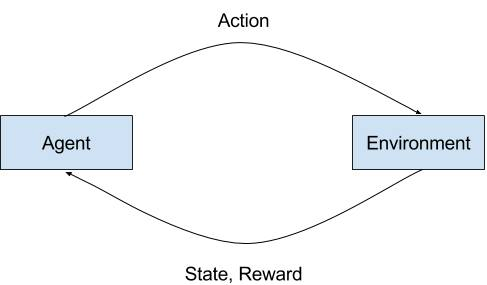
\includegraphics[width=0.5\textwidth]{reinf_learn}
\caption[width=\textwidth]{Representation of general scenario of Reinforcement learning}
\label{fig:reinf_learn}
\end{figure}

The objective of the agent is to maximize his reward and thus to determine the best course of actions, or policy, to achieve the objective. \textbf{However, the information he receives from the environment is only the immediate reward corresponding to the action just taken. No future or long-term reward feedback is provided by the environment.}

\subsection{Exploration vs Exploitation Trade-off}
The agent also faces the dilemma between exploring unknown states and actions to gain more information about the environment and exploiting the information already collected to optimize his reward.

Two main settings are possible:
\begin{enumerate}
    \item Environment model is known to agent. Then the problem is reduced to \textbf{planning}.
    \item Environment model is unknown to agent. Then, he faces \textbf{learning} problem. This will be our main concern.
\end{enumerate}

\subsection{Markov Decision Process Model}
A MDP is defined by:
\begin{enumerate}
    \item Set of states, $S$.
    \item Set of actions, $A$.
    \item Start state, $s_{0} \in S$.
    \item Reward Probability  
    \[P(r_{t+1} | s_{t}, a_{t}) \hspace{0.2cm} where \hspace{0.1cm} r_{t+1} = r(s_{t}, a_{t})\]
    \item State transition probability
    \[P(s_{t+1} | s_{t}, a_{t}) \hspace{0.2cm} where \hspace{0.1cm} s_{t+1} = \delta(s_{t}, a_{t})\]
\end{enumerate}

\begin{figure}[h]
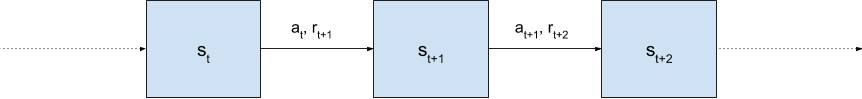
\includegraphics[width=0.5\textwidth]{mdpm}
\caption[width=\textwidth]{Illustration of states and transitions of MDP at different times}
\label{fig:mdpm}
\end{figure}

We also define $\pi:S \rightarrow A$ as the policy function mapping a state S to an action A. In a discrete time model, actions are taken at a set of decision epochs $\left \{ 0, ..., T \right \}$. We deal with infinite horizon i.e. T tends to infinity. Now, the agent's objective is to find a policy that maximizes his expected reward.


\subsection{Policy Value, State-Action Value Function and Q-Learning}
We define the policy value  $V_{\pi}(s)$ in the case of infinite horizon as the expected reward of the agent starting at state $s$ and following policy $\pi$ i.e.
\begin{equation} \label{eq:polVal}
V_{\pi}(s) = E\bigg[ \sum_{\tau=0}^{T-t} \gamma^\tau r(s_{t+\tau}, \pi(s_{t+\tau})) | s_{t} = s \bigg]
\end{equation}
where $T$ tends to infinity.

The policy value  $V_{\pi}(s)$ obey the following system of linear equations (Bellman's equation):
\begin{equation} \label{eq:bellman}
\forall s \in S,\hspace{0.2cm} V_{\pi}(s) = E\big[ r(s,\pi(s))\big] + \gamma \sum_{s^{'}} Pr\bigg[s^{'}|s,\pi(s) \bigg] V_{\pi}(s^{'}) 
\end{equation}
Refer appendix for the proof.

The Bellman's equation can also be written as:
\begin{equation} \label{eq:bellman2}
\textbf{V} = \textbf{R} + \gamma \textbf{PV}
\end{equation}
where,\\ 
$\textbf{P}$ is the state transition probability matrix, 
$\textbf{R} = E[r(s,\pi(s))]$, 
$\gamma$ is the discount for future rewards and $\textbf{V}$ is the unknown policy value matrix

For a finite MDP, Bellman's equation admits a unique solution given by
\begin{equation} \label{eq:bellmanSol}
\textbf{V}_{0} = (\textbf{I}-\gamma \textbf{P})^{-1} \textbf{R} 
\end{equation}
Refer appendix for the proof.

The optimal policy value at a given state $s$ is thus given by 
\begin{equation} \label{eq:optPolVal}
V_{\pi^{*}}(s) = max_{\pi} V_{\pi}(s)
\end{equation}

Finally, we define the optimal state-action value function $Q^{*}$ for all $(s,a) \in S \times A$  as the expected return for taking action $a \in A$ at state $s \in S$ and then following the optimal policy:
\begin{equation} \label{eq:optimalPol}
Q^{*}(s,a) = E\big[ r(s,a) \big]  + \gamma \sum_{s^{'} \in S} Pr\big[  s^{'} | s, a \big]  V^{*}(s^{'}) 
\end{equation}
One can observe that the optimal policy can be given by
\begin{equation} \label{eq:optimalPolObs}
 \forall s \in S,\hspace{0.2cm} \pi^{*}(s) = argmax_{a \in A} Q^{*}(s,a) 
\end{equation}
Thus, the knowledge of the state-vale function $Q^{*}$ is sufficient for the agent to determine the optimal policy, without any direct knowledge of the reward or transition probabilities.

To learn the optimal state-action value function, Q-learning algorithm can be used as shown below:
\begin{algorithm}
\caption{Q-learning Pseudocode \cite{fml}}\label{qlearn}
\begin{algorithmic}[1]
 \scriptsize
\Procedure{Q-LEARNING$\big(\pi \big)$}{}
    \State $\textit{Q} \gets \textit{Q}_{0} $ \Comment{initialization e.g, $\textit{Q}_{0} = 0 $}
    \For{ $\textit{t} \gets 0 \text{ to } \textit{T} $}
        \State $\textit{s} \gets SELECT \textunderscore STATE()$
        \For{each step of epoch $t$}
            \State $\textit{a} \gets SELECTACTION(\pi,s)$ \Comment{Policy $\pi$ from $\epsilon \text{-greedy}$  }
            \State $\textit{r'} \gets REWARD(s,a)$
            \State $\textit{s'} \gets NEXTSTATE(s,a)$
            \State $\textit{Q(s,a)} \gets  \textit{Q(s,a)} + \alpha \big[ r' + \gamma \max_{a'} \textit{Q(s',a')} - \textit{Q(s,a)} \big]$
            \State $\textit{s} \gets \textit{s'}$
        \EndFor 
    \EndFor
    \State \textbf{return} $\textit{Q}$
\EndProcedure
\end{algorithmic}
\end{algorithm}

\section{Deep Reinforcement Learning}
In real world scenarios, the number of states are very large (infinite) which prevents us from representing the state-action value function as a matrix. This is the case with the atari games too. The number of states (configuration of the screen of the game) are infinite and hence, we represent our state-value function using a convolution neural network (instead of a matrix), which takes state-information (screen) as input and outputs scores representing the expected reward corresponding to each action. The optimal action is the one corresponding to maximum score.

So, our optimal state-action value function will be given by
\begin{equation} \label{eq:optStateActionValue}
Q^{*}(s,a;\theta^{*}) = E\big[ r(s,a);\theta^{*} \big] + \gamma \sum_{s^{'} \in S} Pr\big[ s^{'} | s, a;\theta^{*} \big] V^{*}(s^{'})
\end{equation}
where,\\
$\theta^{*}$ represents the learnt parameters of our neural network. Also, the optimal policy is given by 
\begin{equation} \label{eq:optimalPolicyDeep}
\forall s \in S,\hspace{0.2cm} \pi^{*}(s) = argmax_{a\in A} Q^{*}(s,a;\theta^{*})
\end{equation}


\section{Generic Game Playing Agent using Deep-Reinforcement Learning}

\subsection{Model}
Our model is a convolution neural network which takes last 4 preprocessed frames of the screen as input (84x84x4), applies 32 convolution filters with kernel size (8,8) and stride (4,4) and rectifier non-linearity to get first hidden layers of neurons which is further convolved using 64 filters with kernel size (4,4) and stride (2,2) and rectifier non-linearity to get the second hidden layer of neurons which is further convolved using 64 filters with kernel size (3,3) and stride (1,1) and rectifier non-linearity to get third hidden layer of neurons which is fully connected to a layer of 512 neurons with rectifier non-linearity which is again fully connected to output layer of size equal to number of actions in the minimum legal action set. Each output unit represents expected reward obtained by the agent if it performs the action corresponding to that output unit. Here, the preprocessing involves conversion to grayscale and taking the maximum of the value of pixel in current frame and the last frame to avoid flickering effect in the games where some objects occur in even or odd frames only.

\begin{figure}[h]
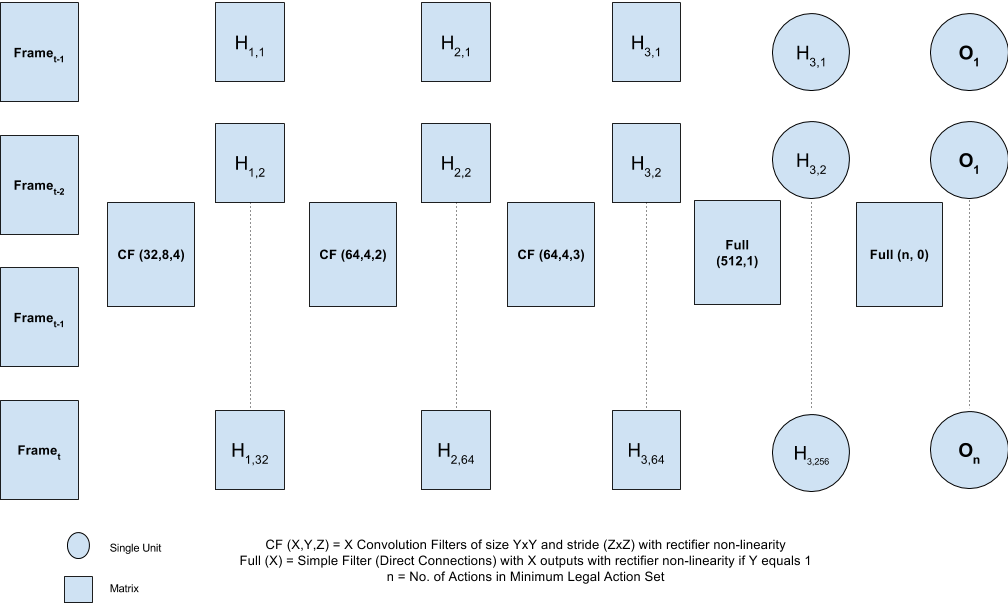
\includegraphics[width=0.5\textwidth]{cnn}
\caption[width=\textwidth]{Convolution Neural Network}
\label{fig:cnn}
\end{figure}



\subsection{Training Details}
The parameter $\epsilon$ in our model simulates the exploration vs exploitation tradeoff. A value of $1$ for $\epsilon$ implies that the agent will make random actions hence explore the environment and a value of $0$ for $\epsilon$ implies that the agent will chooses actions based on the model only and hence exploits the acquired information. While training, we decrease $\epsilon$ with some appropriate decay rate. So, our agent initially starts by making random actions and collects the information in the form of following tuple: ($S_{t}$, $a_{t}$, $r_{t}$, $S_{t+1}$, $g_{t}$) where $S_{t}$ denotes the last four states including the current state, $a_{t}$ denotes the action taken in current state, $r_{t}$ denotes the reward received, $S_{t+1}$ denotes the last four frames including the next state that the agent got into and $g_{t}$ is a boolean denoting whether the game is over or not. Also, the parameters of the convolution neural network that acts as the brain of the agent is initialized with random values. After making a move, the agent selects a random batch of information from the collected information and makes a gradient descent step on the euclidean loss between targets and predictions with respect to network parameters $\theta$ where the inputs and targets to convolution neural network are described below:

Let $j=1,…,m$ represents the indices of the examples in the sampled batch.
Then, input is:
\begin{equation} \label{eq:inputI}
I_{j} = S_{t}^{j}
\end{equation}
and target is:
\begin{equation} \label{eq:inputY}
y^{j} = \left\{\begin{matrix}
r_{t}^{j} & if g_{t}^{j} \text{is true}\\ 
r_{t}^{j} + \gamma max_{a'} Q(S_{t+1}^{j}, a_{t}^{j}; \theta)  &\text{otherwise}
\end{matrix}\right.
\end{equation}

The discount value, $\gamma$ is set to $0.99$. We took a batch size of 32, initial $\epsilon$ value of 1, and final $\epsilon$ value of 0.1. While choosing an action, a uniform random number is generated between 0 and 1. If the generated number is less than $\epsilon$ then a random action is taken otherwise an action prdicted by the state-action value function represented by CNN is taken. We used the rmsprop\cite{rmsprop} version of gradient descent for updating the parameters. A learning rate of $0.00025$, combination coefficient of value $0.95$, momentum of value $0.95$ and minimum squared gradient of value $0.01$ were used in rmsprop.

\section{Results}
Fig. \ref{fig:epochVsReward} shows the epoch number versus the total reward and mean Q-value received by the agent in the atari game \textit{Breakout} during testing. Each test epoch comprises of a fixed number of frames to make the rewards in different epoch comparable. The increase in total reward per epoch shows that our agent learnt to play the game. Fig. \ref{fig:learningCurve} shows the learning curve for the game \textit{Breakout}. As expected, the learning curve doesn't give much insight on whether the agent has learnt to play in an optimal manner while the mean Q-value per epoch does. Then, Fig. \ref{fig:sequenceLearnt}  shows a sequence of frames while the agent has learnt to play the game.
\begin{figure}[h]
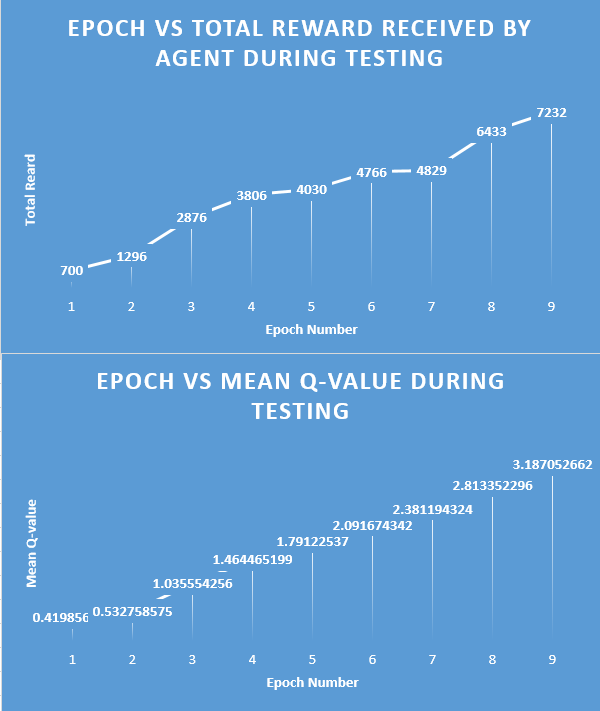
\includegraphics[width=0.5\textwidth]{epochVsReward}
\caption[width=\textwidth]{Epoch number versus the total reward and mean Q-value received by the agent in the game \textit{Breakout} during testing}
\label{fig:epochVsReward}
\end{figure}

\begin{figure}[h]
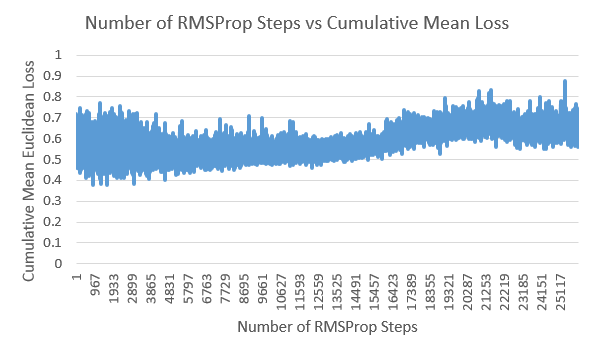
\includegraphics[width=0.5\textwidth]{learningCurve}
\caption[width=\textwidth]{Learning curve for the game \textit{Breakout}}
\label{fig:learningCurve}
\end{figure}

\begin{figure}[h]
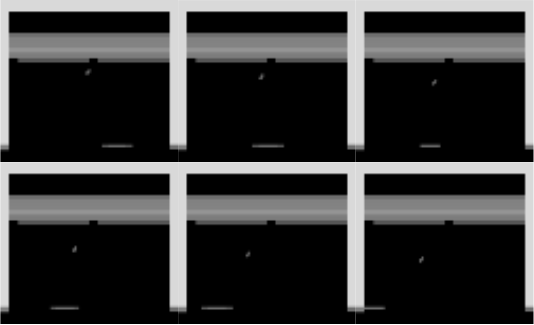
\includegraphics[width=0.5\textwidth]{sequenceLearnt}
\caption[width=\textwidth]{A sequence of frames while the agent has learnt to play the game}
\label{fig:sequenceLearnt}
\end{figure}

\section{Conclusion}
We conclude that our model resembles the way human beings learn to play or act in an environment in the sense that when a positive reward is provided corresponding to an action of an agent in a particular state, then the agent is biased towards making that action in that particular state so as to increase his score by receiving a positive reward. Similarly, the agent avoids to make those actions which results in a negative reward. When the environment is unknown, then a human will try to explore the environment by making random actions from a set of legal actions and this same behaviour is exhibited by our model by making use of the parameter $\epsilon$ as explained in the training details. One can say that the learnt set of parameters represents information relevant for playing the game with respect to which the model is trained. But, there is no way of expressing this information which is in contrast to the way humans learn. We elaborate on this problem in the next section.

\section{Future Work}
Almost all existing machine learning models ignore the availability of (potentially very large) memory. Recently, Reasoning, Attention and Memory (RAM) based models have come into picture where the traditional machine learning models like neural networks are coupled with an external memory component. In RAM-based models, the neural network interacts with this external memory component using an attention mechanism to make inference with reasoning where the reasoning component follows from the way of interaction. We aim to propose an extension of the above model using the ideas of RAM-based models like Neural Turing Machine \cite{ntm} \cite{ntmrl}, Memory Networks \cite{memnn} and End to End Memory Networks \cite{e2ememnn}, so that our complete model/agent gives a reasoning on the action that it makes. For instance, consider the game \textit{Breakout} and the sequence of frames observed by our model in Fig. \ref{fig:sequenceLearnt}.

% \begin{figure}[h]
% 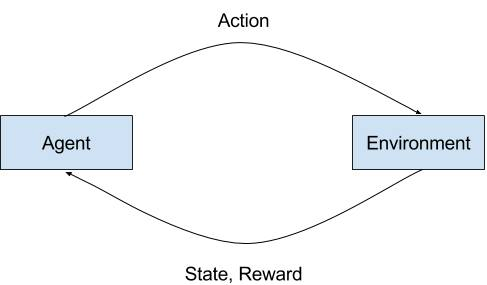
\includegraphics[width=0.5\textwidth]{obsModel}
% \caption[width=\textwidth]{Sequence of frames observed by our model for the game \textit{Breakout}}
% \label{fig:obsModel}
% \end{figure}

Now, our current model/agent moves to the left. But why? A human agent might answer that since the ball is moving towards left the action taken is to move left. This is the part that our current model doesn't answer. It has just learnt some set of parameters that once fitted in the neural network predicts optimal action to take. But hopefully the RAM-based agent will be able to reason that "since the ball is moving towards left, I should also move towards left to prevent death".

\section{Progress of Future Work}
We have implemented the Neural Turing Machine and the End to End Memory Networks in other projects (CS565 and Thesis Project). We are at the stage of designing the extended version of our agent by combining the ideas from Deep Reinforcement Learning, Neural Turing Machine and End to End Memory Networks.



% if have a single appendix:
%\appendix[Proof of the Zonklar Equations]
% or
%\appendix  % for no appendix heading
% do not use \section anymore after \appendix, only \section*
% is possibly needed

% use appendices with more than one appendix
% then use \section to start each appendix
% you must declare a \section before using any
% \subsection or using \label (\appendices by itself
% starts a section numbered zero.)
%


\appendices
\section{Proofs}
\subsection{Proof for Bellman equations}
The policy value  $V_{\pi}(s)$ obey the following system of linear equations (Bellman equations):
\begin{equation} \label{eq:bellmanPolVal}
\forall s \in S,\hspace{0.2cm} V_{\pi}(s) = E\big[r(s,\pi(s))\big] + \gamma \sum_{s'} Pr\big[s'|s,\pi(s)\big] V_{\pi}(s')
\end{equation} 
\textit{\textbf{Proof}}
\begin{equation} \label{eq:step1}
V_{\pi}(s) =  E\bigg[\sum_{\tau=0}^{T-t} \gamma^\tau r(s_{t+\tau}, \pi(s_{t+\tau})) | s_{t} = s  \bigg] 
\end{equation}

\begin{equation} \label{eq:step2}
V_{\pi}(s) = E\big[r(s, \pi(s, \pi(s)) \big] + \gamma  E\bigg[\sum_{\tau=0}^{T-t} \gamma^\tau r(s_{t+1+\tau}, \pi(s_{t+1+\tau})) | s_{t} = s \bigg]
\end{equation}

\begin{equation} \label{eq:step3}
V_{\pi}(s) = E\big[r(s, \pi(s, \pi(s))\big] + \gamma  E\big[ V_{\pi}(\delta(s,\pi(s))) \big]
\end{equation}

The second term in Eqn. \ref{eq:step3} is the second term of Eqn. \ref{eq:bellmanPolVal}

\subsection{Proof of a unique solution of Bellman equation for a finite MDP}
For a finite MDP, Bellman equation admits a unique solution given by
\begin{equation} \label{eq:bellmanSolUnique}
\textbf{V}_{0} = (\textbf{I}-\gamma \textbf{P})^{-1} \textbf{R} 
\end{equation}

\textit{\textbf{Proof}} One just needs to show that $(\textbf{I}-\gamma \textbf{P})$ is invertible and the remaining part is trivial. Note that the infinite norm of P is:
\begin{equation} \label{eq:infiniteNorm}
\norm{\textbf{P}}_{\infty} = \max\limits_{s}  \sum \limits_{s'} \abs{P_{ss'}} = \max\limits_{s} \sum \limits_{s'} Pr\bigg[s^{'}|s,\pi(s) \bigg] = 1 
\end{equation}
This implies that $\norm{\gamma \textbf{P}}_{\infty} = 	\lambda < 1$. The Eigenvalues of $\textbf{P}$ are all less than 1 and $(\textbf{I}-\gamma \textbf{P})$ is invertible.
% use section* for acknowledgement

% Can use something like this to put references on a page
% by themselves when using endfloat and the captionsoff option.
\ifCLASSOPTIONcaptionsoff
  \newpage
\fi




% trigger a \newpage just before the given reference
% number - used to balance the columns on the last page
% adjust value as needed - may need to be readjusted if
% the document is modified later
%\IEEEtriggeratref{8}
% The "triggered" command can be changed if desired:
%\IEEEtriggercmd{\enlargethispage{-5in}}

% references section

% can use a bibliography generated by BibTeX as a .bbl file
% BibTeX documentation can be easily obtained at:
% http://www.ctan.org/tex-archive/biblio/bibtex/contrib/doc/
% The IEEEtran BibTeX style support page is at:
% http://www.michaelshell.org/tex/ieeetran/bibtex/
%\bibliographystyle{IEEEtran}
% argument is your BibTeX string definitions and bibliography database(s)
%\bibliography{IEEEabrv,bibliography}
%
% <OR> manually copy in the resultant .bbl file
% set second argument of \begin to the number of references
% (used to reserve space for the reference number labels box)
%\begin{thebibliography}{1}

%\bibitem{IEEEhowto:kopka}
%H.~Kopka and P.~W. Daly, \emph{A Guide to \LaTeX}, 3rd~ed.\hskip 1em plus
%  0.5em minus 0.4em\relax Harlow, England: Addison-Wesley, 1999.

%\end{thebibliography}

% biography section
% 
% If you have an EPS/PDF photo (graphicx package needed) extra braces are
% needed around the contents of the optional argument to biography to prevent
% the LaTeX parser from getting confused when it sees the complicated
% \includegraphics command within an optional argument. (You could create
% your own custom macro containing the \includegraphics command to make things
% simpler here.)
%\begin{biography}[{\includegraphics[width=1in,height=1.25in,clip,keepaspectratio]{mshell}}]{Michael Shell}
% or if you just want to reserve a space for a photo:

%\begin{IEEEbiography}[{\includegraphics[width=1in,height=1.25in,clip,keepaspectratio]{picture}}]{John Doe}
%\blindtext
%\end{IEEEbiography}

\bibliographystyle{IEEEtran}
\bibliography{IEEEabrv,bibliography}

% You can push biographies down or up by placing
% a \vfill before or after them. The appropriate
% use of \vfill depends on what kind of text is
% on the last page and whether or not the columns
% are being equalized.

%\vfill

% Can be used to pull up biographies so that the bottom of the last one
% is flush with the other column.
%\enlargethispage{-5in}




% that's all folks
\end{document}




%\end{thebibliography}

% biography section
% 
% If you have an EPS/PDF photo (graphicx package needed) extra braces are
% needed around the contents of the optional argument to biography to prevent
% the LaTeX parser from getting confused when it sees the complicated
% \includegraphics command within an optional argument. (You could create
% your own custom macro containing the \includegraphics command to make things
% simpler here.)
%\begin{biography}[{\includegraphics[width=1in,height=1.25in,clip,keepaspectratio]{mshell}}]{Michael Shell}
% or if you just want to reserve a space for a photo:

%\begin{bibliography}
%\blindtext
%\end{bibliography}}

% You can push biographies down or up by placing
% a \vfill before or after them. The appropriate
% use of \vfill depends on what kind of text is
% on the last page and whether or not the columns
% are being equalized.

%\vfill

% Can be used to pull up biographies so that the bottom of the last one
% is flush with the other column.
%\enlargethispage{-5in}


% that's all folks
\end{document}


